

\documentclass[10pt]{article}

\usepackage{amssymb}
\usepackage{amsmath}
\usepackage{amsthm}
\usepackage[pdftex]{graphicx}
\usepackage{multirow}
\usepackage{float}
\newtheorem{thm}{Theorem}



\begin{document}

\begin{center}

{\bf Computing the Log Concave NPMLE for Interval Censored Data}

	\vspace{2mm}

	Clifford Anderson-Bergman, UC Berkeley
	
	cianders@berkeley.edu

	\vspace{2mm}
	
	Yaming Yu, UC Irvine
	
	yamingy@ics.uci.edu

	\vspace{2mm}
	
	Keywords: Interval Censored Data, Shape Constraints, Log-Concave, NPMLE
\end{center}

{\section {Abstract}}

	In analyzing interval censored data, a non-parametric estimator is often desired due to difficulties in assessing model fits. Because of this, the non-parametric maximum likelihood estimator (NPMLE) is often the default estimator. However, the estimates for values of interest of the survival function, such as the quantiles, have very large standard errors due to the jagged form of the estimator. By forcing the estimator to be constrained to the class of log concave functions, we insure a once differentiable survival estimator which has much better operating characteristics than the unconstrained NPMLE without needing to specify a parametric family or smoothing parameter. In this paper, we focus on an algorithm for computing the log concave NPMLE. Using our fast new algorithm, we present evidence from simulated current status data suggesting that the rate of convergence of the log-concave estimator is faster (between $n^{2/5}$ and $n^{1/2}$) than the unconstrained NPMLE ($n^{1/3}$).

{\section{Introduction}}

	The NPMLE is a popular estimator for interval censored data (Turnbull 1976), the main strength being the flexibility of the model. A flexible estimator is especially important for interval censored data, as assessing model fit can be difficult. However, this comes at the cost of high variability of survival estimates. In particular, the convergence rate of the NPMLE has been shown to be $n^{1/3}$ for current status data (Groeneboom 1987) and conjectured to be $ n^{1/3}\log(n)$ for case II interval censored data (Groeneboom 1991). Heuristically, the poor behavior of the NPMLE is due to the fact that the estimated survival curves are similar to step functions with a relatively small number of steps, even for larger datasets (see figure 1).

\begin{figure}[h]
\centerline{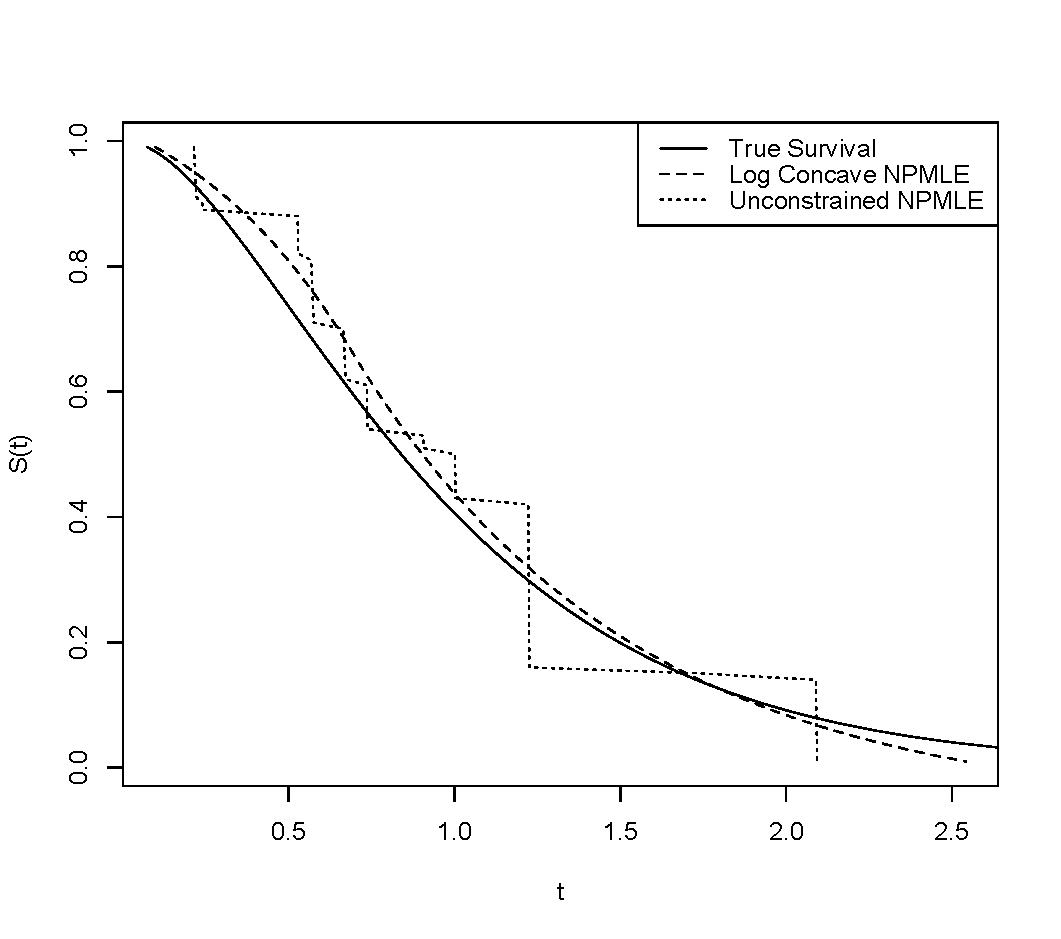
\includegraphics[width = 9cm]{LCvUC.pdf} }
\caption[Log-Concave NPMLE and Unconstrained NPMLE]{Log-concave NPMLE and unconstrained NPMLE. Data are current status data simulated from a Gamma(2,2) distribution with $n = 200$ }
\end{figure} 

	
	Parametric models allow for much more efficient estimation, providing $n^{1/2}$ convergence rates. This depends on parametric assumptions which are hard to assess for interval censored data and can lead to heavy bias in survival estimates if inappropriate. Because of this, parametric models are fairly unpopular for use in interval censored data. 	
	
	Alternatively, issues of the erratic nature of the NPMLE can be remedied by making an assumption about the smoothness of the underlying distribution, rather than making an assumption of parametric family.  This is often done by introducing a smoothness parameter. One method for smoothing with interval censored data is the kernel density estimator (Braun \emph{et al.} 2005), which requires selection of a bandwidth parameter. Another technique is the log-spline density estimator, using a smoothness penalty to select the number of knots (Kooperberg and Stone, 1992). While both of these techniques have been shown to reduce the variance of the estimated survival curve for interval censored data (Pan 2000), they have their drawbacks as well. Both these estimators require selecting an uninterpretable smoothness parameter, which can be non-trivial in the interval censored case. As an example, the logspline density estimator can be found in the CRAN package  ``logspline", with preset smoothing penalties. While this estimator can perform well with light censoring, in our experience with simulated data it behaved poorly under heavy censoring. In particular, it was often observed that either the algorithm fails to converge when used with current status data, even for large data sets (in fact, the estimator appears to perform \emph{worse} for larger data sets). Similar problems were noted in Pan (2000).  Likewise, the question of bandwidth selection for the kernel smoother in application to interval censored data is still an open question. Currently the CRAN kernel smoothing for interval censored data package ``ICE" uses the ad-hoc method of imputing the censored data and using standard uncensored methods for selection of bandwidth. We found that this can lead to heavy bias of the survival estimates in many cases with simulated data.  
	 
	 While both these methods may prove fruitful if automated smoothness parameter selection methods can be developed specifically for interval censored data, in our study we found current implementations of such rules unreliable. This produces demand for a fully automated, theoretically justified smooth estimator. 
		
	We approached this problem by applying a shape constraint on the density function which insures a smooth survival estimate. We applied the popular shape constraint of log concavity (originally published as Bagnoli and Bergstorm 1989, republished as Bagnoli and Bergstorm 2005). A density function $f_X(x)$ is considered log-concave if $f_X(x) = e^{\varphi(x)}$, where $\varphi$ is a concave function. This will insure that $f_X(x)$ will not have more than one peak (but can be flat, such as a uniform distribution). Because a straight line is the boundary of log-concave functions, it insures the tails of the distribution are at most exponential (\emph{i.e.} log-linear). This assumption is considered very flexible as many parametric distributions fit into this category. The families of log-concave distributions include normal, gamma with shape parameter $\ge$ 1, all Weibull densities with exponent $\ge$ 1, all beta densities with both parameters $\ge$ 1 and the logistic density. Non-logconcave distributions include the t-distribution, the lognormal distribution and any multimodal distribution. However, the log-concave estimator has been shown to be useful in mixture modeling (Chang and Walther 2007) so it can be useful for multimodal data as well. This estimator is a consistent estimator of the density in the case of exact data (D\"umbgen and Rufibach 2009) and an efficient algorithm for finding the log-concave NPMLE has been written for uncensored data (D\"umbgen \emph{et al} 2011). 

	Computation of the log-concave NPMLE for interval censored data has been considered in D\"umbgen \emph{et al.} (2011). They present an algorithm which discretizes the domain and  applies an EM algorithm to find an approximation of the log-concave NPMLE (only an approximation due to the discretizing of the data). This algorithm has been implemented in the CRAN package ``logconcens". While this algorithm behaves fairly well for right censored data, it behaves poorly for interval censored data. We found this algorithm frequently failed to converge after 1,000 iterations (default settings on the package set the maximum iterations to 49) and in general, the algorithm was found to be too slow for most purposes (see table 2 for average speeds and frequency of failure to converge). This leads to demand for an fast and reliable algorithm for finding the log-concave NPMLE for interval censored data. 
		
	In this paper, we first provide a  provide a theorem which shows that the log-concave NPMLE can be characterized with a finite number of parameters. Using this theorem, rather than discretizing the data, we construct an efficient method for finding the log-concave NPMLE for interval censored data. This algorithm was found to typically be well over 100 times faster than the algorithm used by the logconcens package and almost never failed to converge after 1,000 iterations ($< 0.1\%$ for simulated data with $n = 500$). In the illustrative example used in this paper ($n = 2,423$), our algorithm was almost 2,000 times faster (0.57 seconds vs 942 seconds). With our new algorithm, we will examine the empirical rate of convergence of survival estimates and compare to those of the unconstrained NPMLE. 
	
	The organization of the rest of this paper is as follows.  In Section 3, we formulate the likelihood function that we are interested in maximizing and state the conditions for which the likelihood function is bounded (proof is provided in the appendix). In Section 4, we prove a theorem which shows that the maximum likelihood can be achieved by a function of a finite number of parameters. In Section 5, we present the different parameterizations that will be used in the algorithm. In Section 6, we discuss the convergence criterion, which is a crucial part of our proposed algorithm. In Section 7, we describe the algorithm itself. In Section 8, we apply the algorithm to a classic sample data set and compare the results to those of the unconstrained NPMLE and the kernel smoother. In Section 9, we compare the rate of convergence of the log-concave NPLME with the unconstrained NPMLE via simulation. In Section 10, we discuss future research topics for the log-concave NPMLE.
	 
	 
{\section {Likelihood Function}}


	We consider the univariate survival scenario and adopt the standard assumption of independent observations among subjects and an independent censoring mechanism. For the $i^{\mathrm{th} } $ subject, suppose the exact event time is known to be within the observation interval $[L_i, R_i]$.  Let $\phi(x)$ represent the log density at time $x$. Because we are dealing with proper density estimates (unlike the unconstrained NPMLE), we must use the standard survival notation of $\delta_i = I_{ \{ L_i = R_i \} }$ (\emph{i.e.}\ $\delta_i$ is an indicator that subject $i$ was uncensored).  Then the log likelihood function is 
	
	\[\ell(\phi) = \displaystyle \sum_{i = 1}^n \delta_i \phi(L_i)   + (1 - \delta_i) \log \left[ S(R_i) - S(L_i) \right]
	\]
	
	where 
	\[
	S(R_i)  - S(L_i) = \int_{L_i}^{R_i} e^ { \phi(x) } \,\mathrm{d}x  
	\]
	
	From this, the log-concave NPMLE is 
	
	\[ \hat \phi =\underset{\phi} {\arg \max} \displaystyle \sum_{i = 1}^n \delta_i \phi(L_i)   + (1 - \delta_i) \log \left[ S(R_i) - S(L_i) \right] 
	\]
	\[
	 \text{which satisfies } \quad \frac{ \phi(x_2) - \phi(x_1)} {x_2 - x_1} \geq \frac{ \phi(x_3) - \phi(x_2)} {x_3 - x_2} \quad \forall x_1 < x_2 < x_3 
	 \]
	 \[ 
	 \text{ and} \int_{-\infty}^{\infty} e^{\phi (x) } \mathrm{d}x = 1
	\]

	To ease the last restriction, we replace $e^{\phi(x)}$ with $\frac{e^{\phi(x)} } { \int_{-\infty}^{\infty}  e^{\phi(x)} \mathrm{d}x}$, so that $e^{\hat \phi(x)}$ is proportional to the log-concave NPMLE. Under this parameterization, the log-concave NPMLE is written as 

	\[ \hat \phi =\underset{\phi} {\arg \max} \displaystyle \sum_{i = 1}^n \delta_i \phi(L_i)   + (1 - \delta_i) \log \left( \int_{L_i}^{R_i} e^ { \phi(x) } \,\mathrm{d}x \right) - n \times \log \left(  \int_{-\infty}^{\infty} e^ { \phi(x) } \mathrm{d}x \right) 
	\]
	\[
	 \text{which satisfies } \quad \frac{ \phi(x_2) - \phi(x_1)} {x_2 - x_1} \geq \frac{ \phi(x_3) - \phi(x_2)} {x_3 - x_2}\quad \forall x_1 < x_2 < x_3 
	 \]
	
	Note that under this parameterization, $\hat \phi(x)$ is calculated up to an additive constant. For simplicity we set $\max_x $ $\hat \phi(x) = 0$. We can then interpret $\hat \phi(x)$ as the estimated log ratio between the density at $x$ and the density at the mode.

	To insure that we can maximize the likelihood, we first show that the likelihood is bounded under minimal conditions.	
	
		\begin{thm}
	\label{thm1}
	The likelihood function is bounded if one of the following three conditions is met:
	
	1. All the data are censored
	
	2. At least two data points are uncensored, and they are not equal to each other
	
	3. There exists one uncensored data point which is not contained in at least one of the censored intervals
	
	
	\end{thm}
	
	See appendix for proof of this theorem. 	
		
{\section{Solution Set}}


	In the case of uncensored observations, it is known that the log-concave NPMLE must be a log piecewise linear function, with knots at the observed times and zero density outside the minimum and maximum observed times (Rufibach 2007). To prove this, consider that for exact times the log likelihood function can be written as	
	\[ \displaystyle \sum_{i = 1}^n \phi(x_i) - n \times \log \int e^{\phi(x)} \mathrm{d}x
	\]
where $x_1<x_2<\cdots<x_n$ are the ordered observations. For a fixed set of values of $\phi(x_i)$, the likelihood is maximized by minimizing $\int e^{\phi(x)} \mathrm{d}x$. For fixed $\phi(x_i)$ and $\phi(x_{i+1})$, $\int_{x_i}^{x_{i+1}} e^{\phi(x)}\mathrm{d}x$ is minimized under the concave restriction of $\phi(x)$ by linearly connecting $\phi(x_i)$ and $\phi(x_{i+1})$. Thus, $\hat \phi(x)$ is a log linear piecewise function in the case of exact observations. The concavity of the log-likelihood function with exact observations insures that the solution is unique.
		
	In the case of interval censored data, the log-concave NPMLE is not necessarily unique. As a trivial example, consider the case n = 1 and the one event is censored. In such a case, any log-concave function which places all of the mass inside of the censored interval would be a log-concave NPMLE. This is very similar to the problem of representational non-uniqueness in the unconstrained NPMLE (Gentleman and Vandal 2002). With such issues in mind, we will instead show that the maximum likelihood can be achieved via a log piecewise linear function with a finite number of knots, while recognizing that there may be other functions which have the same likelihood. 
	
	Define $u$ = number of unique values of $L_i$ and $R_i$. 

	\begin{thm}
	\label{thm2}
	Under the regularity conditions provided in theorem \ref{thm1}, the maximum likelihood for the logconcave NPMLE can be achieved with a piecewise linear function with at most $2u-1$ knots.
	\end{thm}
	
\begin{figure}[h]
\centerline{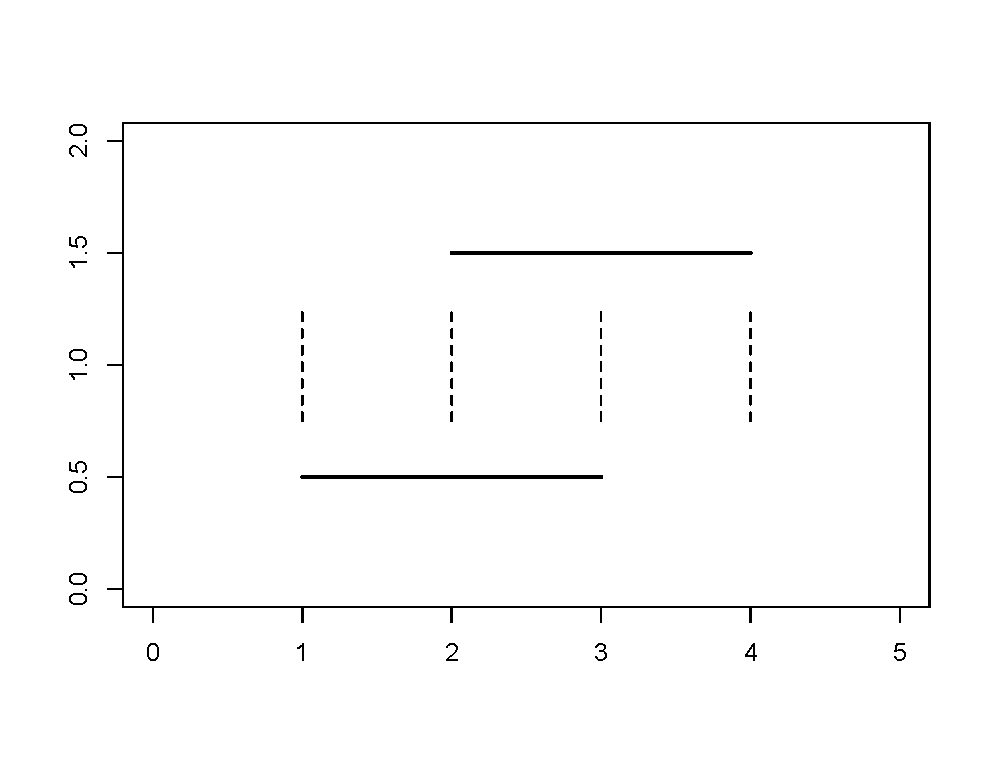
\includegraphics[width = 10cm]{ContrbInt.pdf} }
\caption{Observation intervals and contribution intervals}
\end{figure}	

	\begin{proof}
	
	Let $\hat \varphi$ be a log-concave function which maximizes the likelihood function. We will prove that there exists $\hat \phi$ which is a log linear spline with at most $2u - 1$ knots such that $\ell(\hat \varphi) = \ell(\hat \phi)$.

	Define the $i^{\mathrm{th} } $ observation interval $[L_i, R_i]$ to be the interval in which the $i^{\mathrm{th} } $ event was known to have occurred. Define a contribution interval to be an interval such that both ends of the interval are ends of an observation interval, with no other ends of observation intervals in between. For example, Figure 2 shows two observation intervals, $L_1 = 1$, $R_1 = 3$ and $L_2 = 2$, $R_2 = 4$. This leads to 3 contribution intervals; [1,2], [2,3] and [3,4]. Note that exchanging mass \emph{between} contribution intervals will affect the likelihood function, but exchanging mass \emph{within} will not. 
	
	In any area that is not in a contribution interval, $\varphi(x)$ needs to be minimized for $\hat \varphi(x)$. Thus, $\hat \varphi(x)$ will be linear in areas that are between contribution intervals but are not contribution intervals and $\hat \varphi(x)$ will be $-\infty$ in areas that are not contribution intervals and not between contribution intervals. Therefore, we must only be concerned with whether $\phi$ can replicate the contribution of $\hat \varphi$ to the likelihood function in the contribution intervals while still respecting the constraints.

 	For the $i^{\mathrm{th} } $ contribution interval, define $l_i$ and $r_i$ to be the end points. Let us assume for now that $l_i > -\infty$ and $r_i < \infty$.  For a given $\varphi(l_i)$, $\varphi'(l_i -)$ (left derivative at $l_i$), $\varphi(r_i)$ and $\varphi'(r_i+)$ (right derivative at $r_i$), this contribution interval affects the likelihood only through the total mass assigned to it, \emph{i.e.}\ $p_i = \int_{l_i}^{r_i} e^ {\varphi(x)} \mathrm{d}x$. We define $\hat p_i = \int_{l_i}^{r_i} e^ {\hat \varphi(x)} \mathrm{d}x$
	
	 We will show that for a given $\hat \varphi(l_i)$, $\hat \varphi'(l_i -)$, $\hat \varphi(r_i)$ and $\hat \varphi'(r_i+)$ and $\hat p_i$, by placing one knot between $l_i$ and $r_i$, we can set $\phi(l_i) =\hat \varphi(l_i)$, $\phi'(l_i-) = \hat \varphi'(l_i -)$, $\phi(r_i) = \hat \varphi(r_i)$ and $\phi'(r_i+) = \hat \varphi'(r_i+)$ while $\displaystyle \int_{l_i}^{r_i} e^{\phi(x)} \mathrm{d}x = \hat p_i $
	 
	  Let us define a point inside the contribution interval 	
	
	\[ m_k = \frac{\hat \varphi(r_i) - \hat \varphi'(r_i + ) r_i - \hat \varphi(l_i) + \hat \varphi'(l_i - ) l_i} {\hat \varphi'(l_i - ) - \hat \varphi'(r_i + )}.
	\]		
	In other words, $m_i$ is the location of the intersection of the linear expansions of $\varphi(x)$ from $l_i$ and $r_i$. Of all possibilities of $\varphi$, $p_i$ is maximized by setting $\varphi$ to be linear on the intervals $[l_i, m_i]$ and $[m_i, r_i]$ such that $\varphi(m_i)$ is equal to the height of the intersection of linear extension from each side. We can minimize $p_i$ by setting in $\varphi$ to be linear on $[l_i, r_i]$. This is illustrated in figure 3. 

	\begin{figure}[h]
\centerline{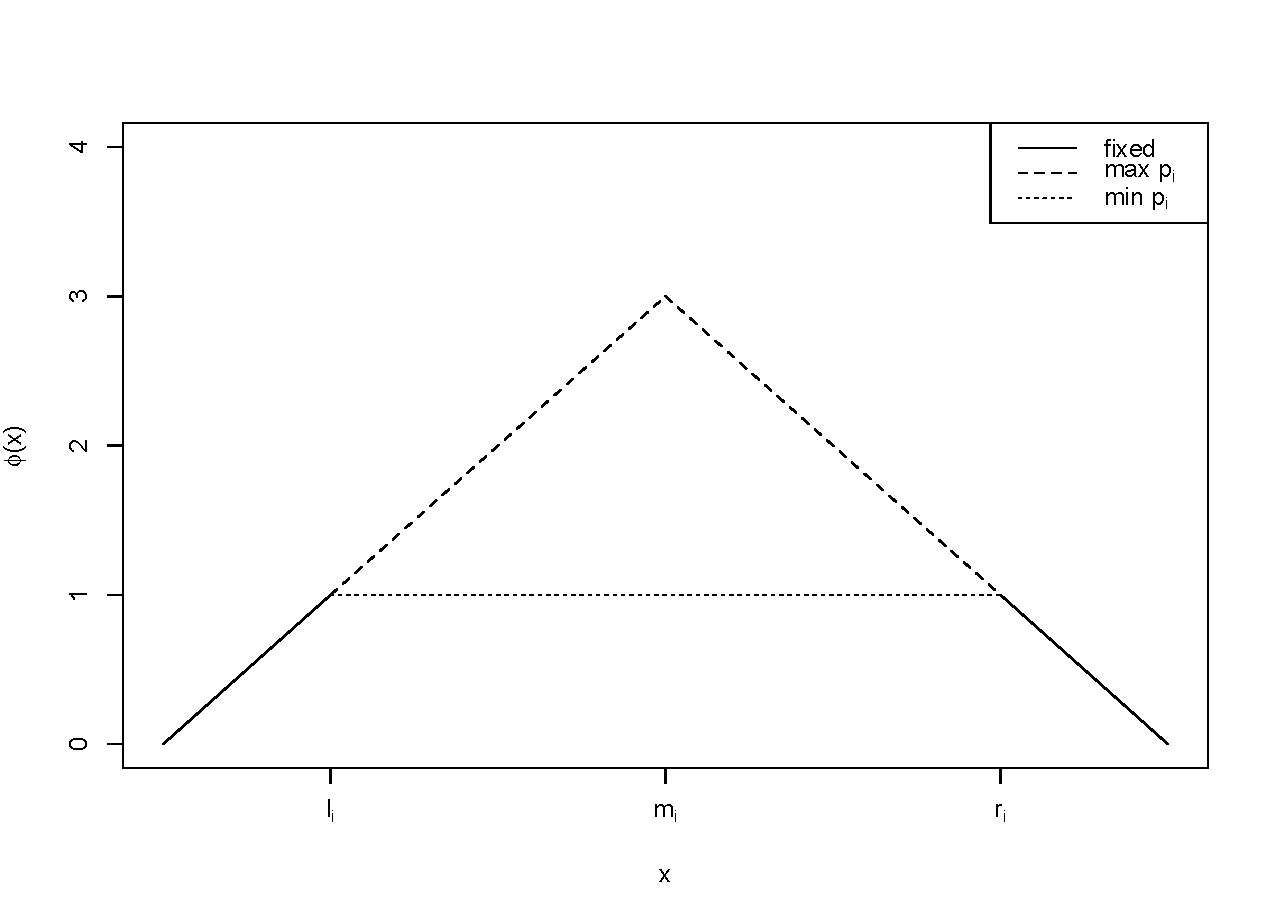
\includegraphics[width = 11cm]{maxminpk.pdf}}
\caption{Maximizing and Minimizing $p_i$}
\end{figure}		

	Therefore, by adding a knot at $m_i$, we can set $p_i$ to either the minimum or the maximum possible under the log concavity constraint, with given $\hat \varphi(l_i)$, $\hat \varphi'(l_i -)$, $\hat \varphi(r_i)$ and $\hat \varphi'(r_i+)$. In fact, we can set $\displaystyle \int_{l_i}^{r_i} e^{\phi(x)} \mathrm{d}x$ to any value between the minimum and maximum of $p_i$ by setting $\phi(m_i)$ to a suitable value between its minimum and maximum allowed by the constraints. In particular, we will be able to set $\displaystyle \int_{l_i}^{r_i} e^{\phi(x)} \mathrm{d}x = \hat p_i$ 

	This does not generalize to the case that $l_i = -\infty$ or $r_i = \infty$, as $m_i$ will not be properly defined by our rule. Let us assume that $r_i = \infty$. In such a case, $p_i$ is maximized by setting $\varphi$ to be linear over $[l_i, \infty)$ with slope equal to $\hat\varphi '(l_i-)$ (if this value is non-negative, we will define $p_i$ = 1). We can minimize $p_i$ by setting the slope equal to $-\infty$ (\emph{i.e.}\ $p_i = 0$). Any value between the minimum and maximum can be achieved by setting this slope to a suitable value between $\hat\varphi '(l_i-)$ and $-\infty$. We can allow $\phi$ to span such choices of slope by setting $m_i = l_i + 1$. Likewise, if $l_i = -\infty$, we can set $m_i = r_i - 1$. 

	This implies any likelihood value which can be achieved by an arbitrary log-concave density can also be achieved by a piecewise log linear function with knots at the end points of contribution intervals and one knot inside each contribution interval. This leads to a maximum of $2u-1$ knots.
	\end{proof}
	
	Theorem~\ref{thm2} is important as it clarifies the form of the NPMLE.  However, without knowing $\hat\phi(x)$, one cannot know the exact location of $m_i$ for the $i^{\mathrm{th} } $ contribution interval. In order to deal with this, $m_i$ is replaced with the fixed location $mid_i = \frac{l_i + r_i}{2}$ for the main portion of the algorithm, as $mid_i$ should be close to $m_i$. Once the solution is sufficiently close, Newton's method will be used to adjust the location of the knots between updates of parameter values. 
		
	For the rest of the thesis, the {\it support set} refers to all end points and mid points of all the contribution intervals.

	{\section{Parameterizations} }
	
	The algorithm presented in this chapter will use an active set algorithm, very similar to the algorithm used in the case of exact times (D\"umbgen \emph{et al}, 2011). In order to clearly define the active set algorithm, several definitions are required. To start with, we define $\beta_i = \phi(x_i)$, where $x_i$ is the $i^{\mathrm{th} } $ ordered support point as described in the theorem above. Let $k$ be the number of support points. Because $\phi(x)$ is a linear spline with knots at $x_i$, the values of $\beta_1, \beta_2, ..., \beta_k$ and $x_1, x_2, ..., x_k$ will completely characterize $\phi(x)$. This will be referred to as the simple parameterization. Occasionally, we will refer to the location of $\beta_i$. This refers to $x_i$. We will also denote $\Delta_i = \frac{\beta_{i+1} - \beta_i} {x_{i+1} - x_i}$. With this notation, we will note that the constraint of log concavity is equivalent to $\Delta_1 \geq \Delta_2 \geq ... \geq \Delta_{k-1}$. In principal, we would like to define $x_i$ to be active if $\Delta_{i-1} > \Delta_i$ and inactive if $\Delta_{i-1} = \Delta_i$. Because round off errors result in inexact calculation of $\Delta_i$, we define $x_i$ to be active if $\Delta_{i-1} > \Delta_i + \xi$ and inactive if $\Delta_{i-1} \leq \Delta_i + \xi$.  We set $\xi = 10^{-13}$ and found no problems resulting from this. 
	
	Similar to the case of exact times (Rufibach 2007), the solution tends to have very few active points compared to the total number of points considered. We can take advantage of this to create an efficient algorithm using an active set parameterization. Under this parameterization, we treat $\phi(x)$ as a linear spline with knots only at the active points and adjust the $\beta_i$'s as such. We use the notation $\beta_i^*$ to denote when we are using the active set parameterization. When using the active set parameterization, if we increase the active parameter $ \beta_i^*$, we also increase the neighboring inactive $\beta_j$'s as though the active points were the only knots of $\phi(x)$  \emph{i.e.}\ the inactive $\beta_j$ are determined by linear interpolation from the nearest active points. To demonstrate this, figure 4 shows adding 1 to $\beta_4^*$. This starts with $\beta_4$ as an inactive point and makes it active as $\phi$ is now kinked at $x_4$ . It also increases the values of $\beta_3$ and $\beta_5$, as they are the surrounding inactive points.  
	
	To formally characterize addition under the active set parameterization, define $a(m)$ to be the index of the $m^{\mathrm{th} } $ active point. If $i = a(m)$ then $\beta_i^{*(t+1)} = \beta_i^{*(t)} + h$ is equivalent to 
		
	\[
	\beta^{(t+1)}_j = 
	\begin{cases}
		\beta^{(t)}_j + h \times \frac{x_j - x_{a(m-1)} } {x_{i} - x_{a(m-1)} } , & \text{if } x_{a(m-1)} < x_j  \leq x_{i} \\ 
		\beta^{(t)}_j + h \times \frac{x_{a(m+1)} - x_j} {x_{a(m+1)} - x_{i} }, & \text{if } x_{ i} < x_j < x_{a(m+1)} \\ 
		\beta^{(t)}_j, & \text{otherwise}
	\end{cases}
	\]

	
\begin{figure}[h]
\centerline{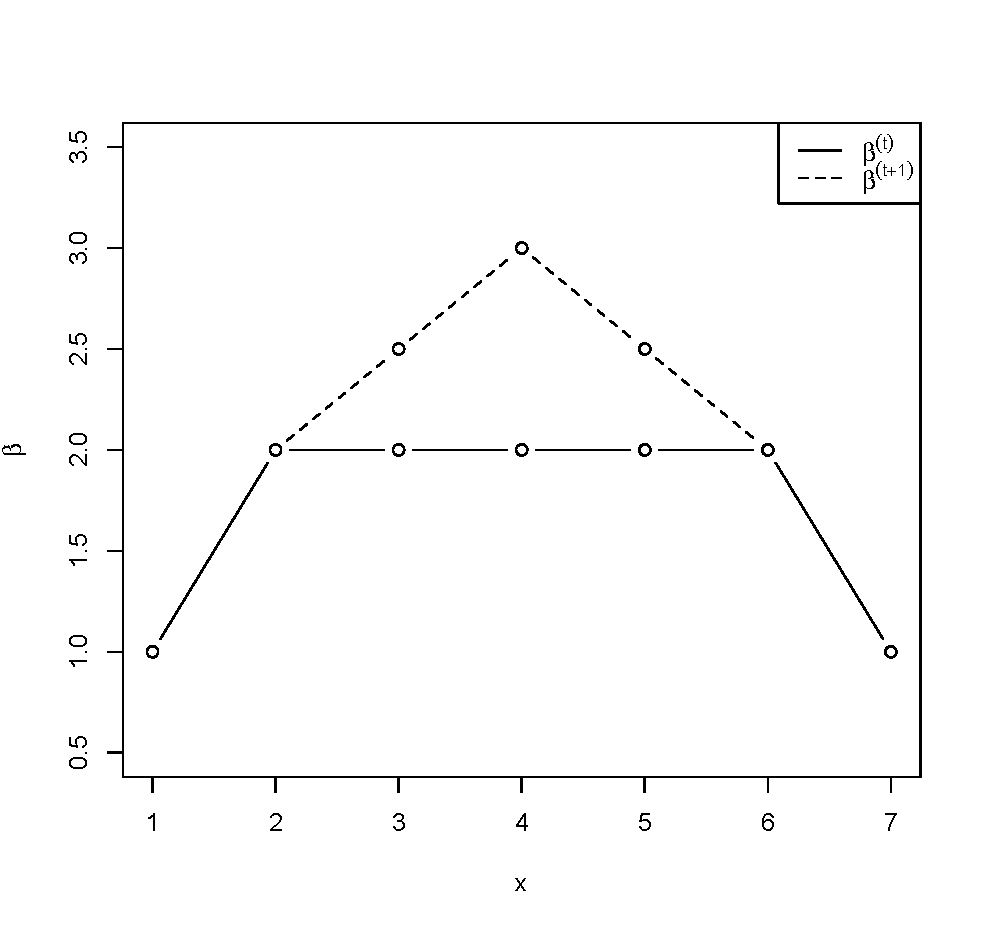
\includegraphics[width = 8cm]{ActivePoint.pdf}}
\caption[Active Set Parameterization: Log-concave]{$\beta_4^{*(t+1)} = \beta_4^{*(t) }+1$}
\end{figure}		
		
	Under the active set parameterization, all active points have a neighborhood for which they can both increase and decrease without violating the condition of log-concavity. Inactive points have a neighborhood in which they can increase and become an active point, but cannot decrease. In the simple parameterization, inactive points cannot decrease and all points can increase only if both neighboring points are active. For example, in figure 4, $\beta_4^{(t + 1)} = \beta_4^{(t)} + 1$ violates log concavity, but $\beta_4^{*(t+1)} = \beta_4^{*(t)} + 1$ does not. 
	
	In a slight abuse of notation, let us also define $\Delta_{a(i)} = \frac{\beta_{a(i + 1)} - \beta_{a(i)} } {x_{a(i + 1)} - x_{a(i)} }$. If $K$ = number of active points, then $\Delta_1 \geq \Delta_2 \geq ... \geq \Delta_{k-1}$ is equal to  $\Delta_{a(1)} \geq \Delta_{a(2)} \geq ... \geq \Delta_{a(K-1)}$. 

			
	{\section{Stopping Criterion} } 
	We discuss the stopping criterion first before presenting the actual iterative algorithm because this discussion clarifies how we characterize the NPMLE, given that it is piecewise log-linear.  Because of the log-concavity constraints, it is natural to consider the KKT conditions (Kuhn and Tucker 1951) which are necessary for an estimate to be a local maximum. Let us define
	
	\[
	\text{KKT error} = {\text{max}} 
	\begin{cases}
		|\frac{\partial \ell } {\partial \beta_i^*}|, & \text{if } \Delta_{i-1} > \Delta_{i} + \xi \\
		\text{max}_i(\frac{\partial \ell}{\partial \beta_i^*},0 ) , & \text{if } \Delta_{i-1} \leq \Delta_i + \xi \\  
	\end{cases}
	\]
	
	In other words, the error is the maximum of the absolute value of the derivatives associated with the active set parameterization of all the active points and the positive derivatives associated with the active set parameterization of the inactive points (because decreasing would violate the log concavity restraint). 
	
	Once the KKT error is below the algorithm tolerance with fixed location of the knots, we allow the location of the knots to move. When this happens, we will have two sources of error: KKT error (it is very likely to increase when the knots move) and error associated with the location of the knots at the active points. Because active points always contain a neighborhood for which the knot can move in either direction, the location error will be the maximum absolute value of the derivative of the log likelihood function as a function of location of each of the active points. This will be referred to as ``location error". At this point in the algorithm, $err$ = max(KKT error, location error). 
	
	The algorithm terminates when either the error is less than the tolerance or the iterations exceed the maximum iterations. We set the tolerance to $10^{-4}$. The reason this value was selected was setting the tolerance to $10^{-5}$ usually required step sizes in the order of $10^{-6}$, which was smaller than the precision of the quadratic programming package we used. If greater precision was desired, the algorithm still achieves this as the univariate step of the algorithm functions properly even for extremely small step sizes. However, this is much more computationally inefficient and it was decided that the increase in precision was not worth the computational cost. In order to check that using tolerance $10^{-4}$ resulted in solutions sufficiently close to the mode, we simulated 200 data sets of size $n = 200$. In each data set, we set tolerance first to $10^{-4}$ and then $10^{-5}$ and compared final likelihoods of our solutions. In these data sets, it was found that the median increase from using tolerance $10^{-5}$ was $1.6 \times 10^{-9}$ and the maximum increase was found to be $2.0 \times 10^{-3}$. 
	
	It is important to note that because the likelihood function is not always concave and potentially could be multi-modal, our stopping criterion is only a necessary condition for the global maximum, not a sufficient condition. However, when the algorithm was started from random starting points, it would always converge to the same solutions, suggesting the issue of potential multi-modality is not too severe.   
	
{\section{Active Set Algorithm} }
	
	{\subsection{Algorithm Outline} } 
	
	
	Each iteration of the algorithm includes four steps: one which selects new points to add to the set of active points (similar to the VDM algorithm of Fedorov 1972), one which efficiently increases the likelihood over the set of currently active points (similar to the methods used to compute the log-concave NPMLE with exact observations found in D\"umbgen \emph{et al.} 2011), one that fixes the tails and one that moves the location of the active points. The first step selects the index $i$ with the maximal error and uses simple univariate techniques to find an optimal $\beta_i^*$. The second step optimizes over the active set proceeds by approximating the log-likelihood function with a second order Taylor expansion, and then maximizing this approximation using quadratic programming, similar to the ICM algorithm (Jongbloed 1998).  Because often $\beta_i = -\infty$ on the tails at the solution, it is occasionally necessary to adjust the tails of $\beta$ for numerical stability which is done in the fixing tails step. Finally, after the solution is sufficiently close, we allow the location of the active points to move via Newton's method. The basic form of the algorithm is as follows.
	
	\vspace{3mm}
	
	\begin{itemize}
	
		\item Set initial values for $\beta$ 
		
		\item Set MOVEX = FALSE
		
		\item While ($err > \epsilon$ and $t <$ max iterations)
		
		\{
		
			\begin{itemize}
			
			\item Set $t = t + 1$
			
			\item Select index $i$ with maximal KKT error
			
			\item Use univariate optimization to update $\beta_i^*$
						
			\item Use quadratic programming to optimize over active set
			
			\item Fix tails of $\beta$ if necessary
			
			\item Calculate $err$ = KKT error
			
			\item If($err < \epsilon$)
				
				\begin{itemize}
				
				\item MOVEX = TRUE
				
				\end{itemize}
			
			\item If(MOVEX == TRUE)
				
				\{
				
				\begin{itemize}
										
				\item Use bivariate Newton's method to update knot location of active points which are mid points
				
				\item Calculate $err$ = max(KKT error, location error)
				
				\end{itemize}
			
				\}
			
			\end{itemize}
			
	\}
	
	\item Convert $\beta$ to $e^{\phi(x)} / \int e ^ {\phi(x)} \mathrm{d}x$
	
	\item Return $e^{\phi(x)} / \int e ^ {\phi(x)}\mathrm{d}x$
	
	\end{itemize}
	
	It is important to note that after the MOVEX part of the algorithm is activated, we will still need to update all values of $\beta_i$, as moving the location of the knots will have a change in the constraints. Because of this, when we calculate $err = \text{max(KKT error, location error)}$, we must recalculate the KKT error rather than reusing the earlier calculated KKT error in the earlier step of the algorithm. 
	
	There is one technical note about the initial values of $\beta$. It is very tempting to start with a uniform set, \emph{i.e.} $\beta_1 = ... = \beta_k = 0$. However, if the censoring is over an infinite area ($R_i = \infty$ or $L_i = -\infty$), this will result in an improper distribution, as the distribution Uniform$(a, \infty)$ is improper. To insure the initial distribution is properly defined, we set $m$ = $\frac{k + 1} {2}$ and set $\beta_i = -|x_m - x_i | / \sigma_x^*$, where $\sigma_x^*$ is the standard deviation of all finite support point locations. This leads to a Laplace distribution if defined on $\mathbb{R}$ and a truncated Laplace distribution otherwise.	
	{\subsection{Univariate Optimization}} 
	
	Our algorithm selects the index $i$ associated with the maximum KKT error. Once the index $i$ is selected, $\beta_i^*$ must be selected which increases the likelihood. Let $i = a(j)$ (if $i$ is not an active point, it will be after optimization). From the constraints $\Delta_{a(j-2)} \geq \Delta_{a(j-1)}$, $\Delta_{a(j-1)} \geq \Delta_{a(j)}$ and $\Delta_{a(j)} \geq \Delta_{a(j+1)}$, we derive the constraints
	
	\[ \beta_i^* \leq \text{min}\left(\beta_{a(j-1)} + \Delta_{a(j-2)} \times (x_{a(j)} - x_{a(j-1)}), \beta_{a(j+1)} -\Delta_{a(j+1)} \times (x_{a(j+1)} - x_{a(j)}) \right) 
	\]
	
	\[ \beta_i^* \geq \left(\frac{1}{x_{a(j+1)} - x_{a(j)}} +  \frac{1}{x_{a(j)} - x_{a(j-1)} } \right)^{-1} \times \left(\frac{\beta_{a(j+1)} } { x_{a(j+1)} - x_{a(j)}} + \frac{\beta_{a(j-1)}} {x_{a(j)} - x_{a(j-1)} } \right)
	\]
	
	Constraints which involve an undefined index, such as $a(0)$, can be ignored. If $\frac{d^2 \ell} {d (\beta^*_{i})^2 } < 0$, then Newton's method was used, subject to the above constraints. Half stepping was used to insure monotonic convergence. Rarely it was observed that $\frac{d^2 \ell} {d (\beta^*_{i}) ^2 } \geq 0$, in which case the bisection method was used to update $\beta^*_i$. Although $\ell(\beta^*_i)$ was observed to be non-concave, it was not observed to be multimodal.
	
	Much like the VDM algorithm, these steps alone insure that the algorithm will reach a local maximum, but is observed to do so very slowly. Using simulated data with $n = 200$, we observed that using these steps alone frequently failed to meet the convergence criterion after 1000 iterations, implying that an algorithm based only on univariate optimization would be insufficient. In section 7.3, we present a step that updates all active points simultaneously and greatly accelerates the algorithm. While the multivariate step can be forced to never decrease the likelihood function, the multivariate step alone is not insured to find a local maximum. Thus, we will include both the univariate and multivariate steps in our algorithm to insure convergence. 
	
	{\subsection{Maximizing Over an Active Set} }
	
	Once given an active set of points, we need a step which can  maximize over the active set efficiently. Because of the linear constraints of concavity, Newton's method is difficult to apply as it would not respect the boundaries. Instead, an ICM (Jongbloed 1998) algorithm is used to maximize the over the active set, similar to the algorithm used in the exact case (D\"umbgen \emph{et al.}, 2011). An ICM algorithm works by approximating the target function with a second order Taylor expansion, in which the off diagonal partial derivatives are ignored. In this application, the parameters considered will be the log density at the active points, \emph{i.e.} $\beta_i$'s. It is worth noting that in the traditional ICM algorithm, the off diagonals are ignored due to the expense of computation. In this case the number of parameters considered  is actually fairly low, making the number of off diagonals more manageable, but we have other reasons to ignore the off diagonals which will be discussed shortly. This approximation is maximized, according to the linear constraints, via quadratic programming. We will use the notation that a quadratic program minimizes
	
	\[ \frac{1}{2} d^T Q d + c^T d
	\]
	
	Under the constraint \[ A d \leq b\]
	
	Because quadratic programming minimizes a program, we will minimize the Taylor approximation of $-\ell(\beta^*))$, with the off diagonals of the Hessian ignored. In order to have $\frac{1}{2} d^T Q d + c^T d$ be the given approximation, we define
	
	\[ d_i = \beta^{*(t+1)}_{a(i)} - \beta^{*(t)}_{a(i)}
	\]
	
	\[Q_{i,i} = - \frac{\partial^2 \ell(\beta^{*(t)} )} {\partial {\beta^{*(t)}_{a(i)}}^2}
	\]
	 
	 \[
	 Q_{i,j (i\neq j)} = 0
	 \]
	 
	\[c_i = -\frac{\partial \ell(\beta^{*(t)})} {\partial \beta_{a(i)}^{*(t)} }
	\]
	
	In order to preserve the constraint of $\Delta_{a(i)} \geq \Delta_{a(i+1)}$, we set 
	
	\[ A_{i,i} = \frac{1}{x_{a(i+1)} - x_{a(i)} }
	\]
	
	\[ A_{i, i + 1} = \frac{-1}{x_{a(i+1)} - x_{a(i)} } + \frac{-1}{x_{a(i+2)} - x_{a(i + 1)} }
	\]
	
	\[ A_{i, i + 2} = \frac{1}{x_{a(i+2)} - x_{a(i + 1)} }
	\]
	
	\[ b_i =\Delta_{a(i + 1)}^{(t)} - \Delta_{a(i)}^{(t)}
	\]
	
	Similar to the ICM algorithm (Jongbloed 1998), half steps will be taken to insure the likelihood function does not decrease. In other words, if $\ell ( \beta^{*(t)} + d ) < \ell ( \beta^{*(t)}  ) $, then $d$ is replaced with $d/2$ until $\ell ( \beta^{*(t)} + d ) \geq \ell ( \beta^{*(t)} )$. It was observed that these half steps were required very infrequently. However, if the tolerance was set very low, such as $10^{-6}$, often this step would fail to increase the likelihood function, as the tolerance for the quadratic solver appeared larger than the necessary step size (the ``solve.QP" function from the R package ``quadprog" was used. Failure typically happened when the largest component of $d$ (before half stepping) was on the order of $10^{-6}$. In such cases, the univariate steps would still work). 
	
	Perhaps the most novel part of this algorithm is in how we deal with the fact that $\ell(\beta^*)$ may not be locally concave. In particular, the quadratic function used to approximate the likelihood function will be unbounded if the Hessian is non-negative definite, leading to a degenerate purposed step. Because the ICM algorithm ignores the off diagonals of the Hessian matrix, the only case of concern is when the diagonals of the Hessian are not negative (when the off diagonals are included in the quadratic approximation of the likelihood function, the Hessian was more likely to be non-negative definite). In order to remedy this, an approximation to the second derivative was used which would be insured to be negative. This approximation takes advantage of the fact that the likelihood function is bounded from above. 
		
	Suppose that the likelihood function is not locally concave as a function of one of the active points, \emph{i.e.}\ $ \frac{\partial^2 \ell} { \partial {(\beta^{*(t)}_{a(i)})}^2} \geq 0$. Let $\tilde \beta^*_{a(i)}$ be the value of $\beta^*_{a(i)}$ that maximizes $\ell(\beta^*_{a(i)})$ in the direction of $ \frac{\partial \ell} {\partial \beta^{*(t)}_{a(i)}} $ (\emph{i.e.}\ if $  \frac{\partial \ell} {\partial \beta^{*(t)}_{a(i)}} > 0$ only consider  $\tilde \beta^*_{a(i)} > \beta^{*(t)}_{a(i)}$, and if $  \frac{\partial \ell} {\partial \beta^{*(t)}_{a(i)}}< 0 $ only consider $\tilde \beta^*_{a(i)} < \beta^{*(t)}_{a(i)}$)  with all other $\beta_{a(j)}$ held fixed. It is worth noting that we don't require $\tilde \beta^*_{a(i)}$ to respect the boundary set by the constraint of log concavity. If we then consider approximating $\ell(\beta^*_{a(i)})$ with a quadratic function whose first derivative at $\beta^*_{a(i)}$ is $  \frac{\partial \ell} {\partial \beta^{*(t)}_{a(i)}} $ and whose maximum is reached at $\tilde \beta^*_{a(i)}$, this would imply that our approximation of the second derivative would be
	
	 \[\frac{- \left( \frac{\partial \ell} {\partial \beta^{*(t)}_{a(i)} }  \right) } {\tilde \beta^*_{a(i)} -\beta^{*(t)}_{a(i)}}
	 \]
	 
	 This is guaranteed not to be positive.
	
	In the case of a concave likelihood function, half stepping insures that the likelihood function will increase. Because our target function is not locally concave when using this approximation, even half stepping does not insure the likelihood function will increase. If after sufficient half steps (we chose 5), the likelihood still does not increase, this step of the algorithm is skipped. Theoretically, if the ICM step repeatedly failed, the algorithm could be extremely slow due to relying only on the univariate optimization. However, this was not observed to occur and substituting this approximation into the ICM algorithm appears to work very well, usually reducing the number of iterations required to below 100 for simulated data of size $n = 200$. While finding  $\tilde \beta^*_{a(i)}$ does come with some computational cost, this approximation was required infrequently and could be done efficiently enough that the computational costs were not significant in the speed of the algorithm. 
	
		{\subsection{Moving the Knots} } 
	
	Recall that we used $mid_k$ as the location of the knots in the center of each contribution interval because we don't know the exact location defined as $m_k$ in our theorem. To optimize the position of the knots, a bivariate Newton's method was used, with half-stepping of proposed steps to insure the new proposed estimate increases the likelihood function and respects the constraints. The two parameters considered were the location of the knot (\emph{i.e.}\ $x_i$) and the log density at the knot (\emph{i.e.}\ $\beta_i$). While the log likelihood function does appear consistently to be concave as a function of the location of the knots, we already know that the log likelihood is not always concave as a function of $\beta_i$. In the case where the Hessian matrix is not negative definite, we will perform Newton's method on only the location of the knot and not update $\beta_i$ in this step (as it will updated in the other steps of the algorithm). The algorithm includes a bisection step for knot location, should the likelihood function be non concave as a function of the knot location, but we have not observed it to be necessary. 
	
	It was found that the most computationally efficient way to implement this moving of the knots was to first let the algorithm run without moving the knots until the KKT error was below the tolerance. Once this occurred, then we would add the bivariate Newton's method into the algorithm, alongside both the univariate and the ICM steps, until both the KKT error and location error were below the tolerance. Once this was satisfied, the algorithm was considered converged. 
	
		{\subsection{Fixing the Tails} }
	
	When computing the log-concave NPMLE with exact observations, the area which must have positive mass is known in advance (\emph{i.e.}\ the range of all observed times). When computing the log-concave NPMLE for interval censored data, this not the case, as there are often contribution intervals which receive 0 mass at the log-concave NPMLE. A trivial example to consider is if the data consisted of two overlapping intervals. The log-concave NPMLE would place all the mass in the overlap and no mass to the other two surrounding contribution intervals.% In the case of the unconstrained NPMLE, the mass is known to be positive only in the set of Turnbull intervals. However, the log-concave constraint implies that this is not the case and often some of the contribution intervals outside of the minimum and maximum Turnbull intervals will receive positive mass at the log-concave NPMLE, while others will not.
	 		
	Because of this, simply allowing the earlier steps to find the log densities	 at the tails of the estimated density can lead to numerical instability as $\beta_i \rightarrow -\infty$. Numerical instability typically happened in the range of $\beta_i = -1000$ for some $i$, as derivatives and second derivatives approached 0.% Even if numerical issues were not observed, allowing the algorithm to meet the stopping criterion can be very computationally expensive for a rather trivial transformation of $\phi(x)$. 
	
	To cope with this, our algorithm would periodically check if setting $\beta_i$ to $-\infty$ increases the likelihood for on the tails (\emph{i.e.} $i$ is either the smallest or largest value of $i$ such that $\beta_i > -\infty$) if $\beta_i < -t$ for some threshold $t$. If this increased the likelihood, the $\beta_i$ associated would be set to $-\infty$ and either $\beta_{i+1}$ or $\beta_{i-1}$ (depending on which tail) would be checked next. If setting $\beta_i = -\infty$ did not increase the likelihood, the values would remain unchanged and this part of the algorithm would terminate. Interestingly, choosing $t$ too small leads to local maxes which can be considerably less than the global max, even if optimization techniques are used to check if adding mass back to the tails which have been set to $-\infty$ could increase the likelihood. For poorly chosen $t$, such as $t = 1$, the difference in log likelihood was observed to be as high as 1.5 and the mass could be significantly different on the tails, despite the convergence criterion being satisfied. On the other hand, setting very large $t$, such as 500, was found to increase the number of iterations required several fold. Fortunately, there appears to be a large region for choices of $t$ such that neither issues occurred. The performance across $t$ = 1, 5, 10, 20 and 40 was examined. While it was found that $t = 10$ appeared satisfactory, for robustness $t = 20$ was selected as it led to a small increase in average iterations (about 15\% more). With this fix, it was found that even with random starting values, the algorithm only led to the same estimate. 
		
		{\section{Algorithm Speeds} } 
	
	To investigate the speed of our algorithm, we computed the log-concave NPMLE across different scenarios. The complexity of each step of the algorithm is not a function of sample size, but rather the number of unique times in the data. Each step is of order $O(u^2)$, where $u$ is the number of unique times. While given $u$, $n$ does not affect the complexity of each iteration,  we see that the number of iteration increases with $n$ for a fixed $u$. Empirically, it appears the number of iterations required may be of order $O(\sqrt{n})$. On Table 1, we present average computation time in seconds across different sample sizes and different numbers of unique times in the data using simulated current status data in which both the event time and inspection time was simulated from gamma(2,2) distribution. Binning was used to create the number of unique times. 
	
	\begin{table}[H]

\begin{center}	
\caption[Average Computation Times for our Algorithm]{Average computation times in seconds for our algorithm. ``-" implies combination of $n$ and $u$ is invalid (i.e. $u > n$) }
\begin{tabular} {| c | c | c | c | c | c | c | c |} 


	 \hline

		 & \multicolumn{7} {|c|} {Unique Times} \\
		
	\hline	
		
	$n$ & 10 & 50 & 100 & 500 & 1000 & 2000 & 5000\\	
		
	 \hline 
 
 	100 & 0.07 & 0.15 & 0.17 & - & - &  - & -\\ 
	
	\hline
	
	500 & 0.19 & 0.27 & 0.46 & 0.86 & - & - & -\\
	
	\hline
	
	5000 & 0.42 & 0.86 & 1.11 & 5.07 & 7.59 & 31.6 & 156\\ 
	
	\hline
	
\end{tabular}
\end{center}

\end{table}

	We compared this to the R package logconcens. We found that the algorithm in logconcens frequently failed to converge. We simulated datasets in the same manner as above, except that we only considered sample sizes $n$ = 25, 50 and 100. In addition to average times, we present the proportion of datasets for which the algorithm failed to converge after 1,000 iterations. 
	

	\begin{table}[H]
	
	\label{LogConSpd}
	
\begin{center}	
\caption[Average Computation Times for Logconcens Algorithm]{Average computation times in seconds for logconcens. Values in parentheses are proportion of datasets failed to converge after 1,000 iterations}
\begin{tabular} {| c | c | c | c |} 


	 \hline

		 & \multicolumn{3} {|c|} {Unique Times} \\
		
	\hline	
		
	$n$ & 10 & 25 & 50 \\
		
	 \hline 
 
 	25 &    9.29 (0.26)	& 20.4 (0.37)	& -	\\ 
	
	\hline

 	50 &  14.0 (0.15)  	& 21.7 (0.27)	& 47.9 (0.67)   \\ 
	
	\hline
	
 	100 &  16.9 (0.20)  	& 37.1 (0.43)	&  56.1 (0.47)	   \\ 
	
	\hline
	
\end{tabular}
\end{center}

\end{table}


	
		
	{\section{Illustrative Example} }
	
	For a illustrative example, we will borrow data from MacMahon and Worcestor (1966). Questionnaires were collected from $n = 2423$ participants regarding age at menopause. Because several of the subjects had not experienced menopause yet, this data set contained right censored data. However, MacMahon and Worcestor (1966) found that there was a marked terminal digit clustering in the response of reported time of menopause. Because of this, Krailo and Pike (1983) recommended only using the menopausal status of women at the time of the questionnaire, thus resulting in current status data. The data also contains two types of menopause; operative menopause and natural menopause. 
	
	Earlier analyses of this data used a competing risks model (Jewell \emph{et al.} 2003). For demonstrative purposes, we will only examine the time to menopause, regardless of the type of menopause. For this example, we will examine the estimated densities and survival curves, although clearly it would be simple to also examine the estimated hazard as well. We wanted to compare the log-concave estimate to the unconstrained NPMLE, the logspline estimator and the kernel density estimator. However, using the standard settings found in the CRAN logspline package, the logspline estimator failed to converge with this dataset, a common problem for the logspline estimator with current status data. When using the kernel smoother, the problem of selecting bandwidth was non trivial. Braun \emph{et al.} (2005) suggest using cross validation for selecting bandwidth. With a dataset of this size and current software options for the kernel smoother, this is not an option. Instead, midpoint imputation was used to determine bandwidth, as demonstrated in the CRAN ICE package. Other ad hoc fixes used were left endpoint and right endpoint imputation. All of these lead to relatively close bandwidths, which lead to very similar estimates. 
		
\begin{figure}[h]
\centerline{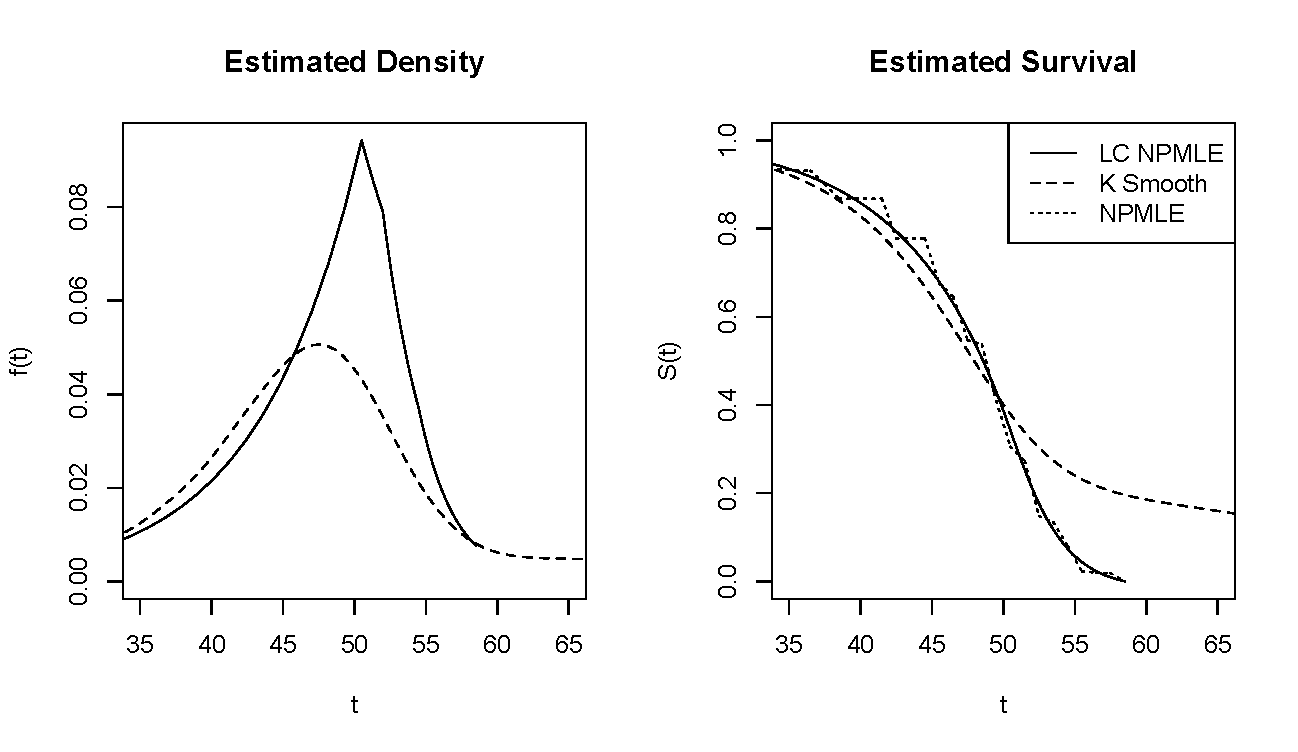
\includegraphics[width = 12cm]{MenoPlot.pdf}}
\caption{Estimated Functions}
\end{figure}		
	
	Plotted estimates can be seen in figure 5 for the menopause data. We see is that the log-concave NPMLE has a much more jagged density estimator than the kernel smoother. This can be seen as a disadvantage for the log-concave NPMLE where smoothness of the estimated density is a priority. There is no unconstrained NPMLE density estimate, as the unconstrained NPMLE does not provide valid density estimates. We also note that while the log-concave NPMLE and the unconstrained NPMLE survival estimates appear consistent with each other, there is a large disagreement with those estimates and the kernel smoother's. The log-concave NPMLE places 0 masses beyond t = 58.5, while the kernel smoother places mass as far as t = 100. The NPMLEs appear to agree with what is known about menopause, while the kernel smoother appears to be a less accurate portrayal of the distribution of time to menopause. For example, Treloar 1981 presents data from a longitudinal study. Excluding the cases lost to follow up, all 729 cases had experienced menopause by age 59 (and only one had experienced menopause after 58). However, the kernel smoother estimates that $S(59) =  0.19$. In contrast, both the log-concave NPMLE and unconstrained NPMLE place 0 mass beyond 58.5, which agree much better with Treloar's findings. The bias of the kernel smoother is likely due to an inappropriate chose of bandwidth, although post-hoc adjustment of the bandwidth did not fix this until the bandwidth was so small that the estimated survival curve was no longer smooth. 
	
	 The current implementation of the LC NPMLE algorithm took 0.57 seconds (221 iterations) to converge. The algorithm in the logconcens package took 942 seconds to converge. The kernel smoother took 16.5 seconds and the unconstrained NPMLE algorithm, as implemented in the CRAN package  MLEcens, took 0.139 seconds to converge. 
	
	
	{\section{Empirical Rates of Convergence} } 
	
	The unconstrained NPMLE has been shown to have theoretic cube root convergence. Although we do not attempt to derive the theoretic limiting distribution of the log concave NPMLE in this work, we used our algorithm to inspect the empirical rate of convergence via Monte Carlo simulation. In particular, we assume that
	
	\[ ( \hat F (t_0) - F(t_0) ) n^{\beta_1} \rightarrow U_1 \]
	
	and
	
	\[ (\hat F^{-1}(p_0) - F^{-1}(p_0) ) n^{\beta_2} \rightarrow U_2 \]
		
	where $U_1$ and $U_2$ are fixed distributions. Under this assumption, we note that 
	
	\[ \sigma_i (n) \approx c_i \times n^{-\beta_i} \text{ and}	\]
		
	\[ \log( \sigma_i (n) ) \approx \log(c_i) - \beta_i \log(n) \text{, \emph{i} = 1,2} \]	
		
	where $\sigma_i(n)$ is the standard deviation of either $\hat F(t_0)$ or $\hat F^{-1}(p_0)$. 	
	
	To estimate $\beta_1$ and $\beta_2$, we estimated $\sigma_i(n)$ across a range of values for $n$ via simulation and used linear regression on the log transformed values. We used sample size $n = 100$, 200, 400, 800, 1,600, 3,200, 6,400 and 12,800. At each sample size, we used 1,000 simulations to estimate $\sigma(n)$.  We did this both for the log concave NPMLE and the unconstrained NPMLE, although theory dictates that the rate of convergence for the unconstrained NPMLE should be $1/3$ for current status data.  
	
	In each simulation, we used a current status censoring mechanism with $C_i \sim $ uniform(0,1). We considered two different scenarios for the event time: $T_i \sim $ uniform(0,1) and beta (5,5). This was to illustrate our findings that the rate of convergence differed depending on whether the event time distribution was on the boundary of log-concave distributions (\emph{i.e.} uniform(0,1)) or not on the boundary (\emph{i.e.} beta(5,5) ). We inspected the standard deviations of $\hat F(t_0 = 0.5)$ and $\hat F^{-1}( p_0 = 0.5)$.
		
	From table 3, we see the estimated rates of convergence for both the log concave NPMLE (LC NPMLE) and unconstrained NPMLE (UC NPMLE). For the unconstrained NPMLE, we see that the empirical rate of convergence is fairly close to the theoretical rate of 1/3 in all scenarios. For the unconstrained NPMLE, the rate of convergence appeared slightly lower when the event time was well inside the boundary, although still significantly higher than the rate of convergence one the unconstrained NPMLE. This result is consistent with many other exploratory simulations we conducted but did not list in this paper. Our findings suggest that the rate of convergence is dependent on the distance (not properly defined at this time) between the event time distribution and the log concave boundary. Further theoretically derived results would be very helpful for analyzing the advantage gained by using the shape constrained estimator for interval censored data. At this time, we are not aware of any work being done in that area. 

	All the estimated standard deviations can be found in table 4 in the appendix.
	
\begin{table}[H]
	
\label{EstConRates}
		
\begin{center}	
\caption[Test]{Estimated Rates of Convergence, values in parenthesis = 95\% CI}

\vspace{1mm} 
\begin{tabular} {| c | c | c |} 


	\hline	
		
	Scenario							& 	LC NPMLE 		& 	UC NPMLE  \\
	\hline	
	
$\hat F(0.5), T\sim \text{unif(0,1)}$		&	-0.51 (-0.51, -0.50)	&	-0.34 (-0.36, -0.33) \\


$\hat F^{-1}(0.5), T\sim \text{unif(0,1)}$	&	-0.48 (-0.49, -0.47)	&	-0.32 (-0.33, -0.31) \\
	
	\hline
	
$\hat F(0.5), T\sim \text{beta(5,5)}$		&	-0.43 (-0.44, -0.42)	&	-0.34 (-0.36, -0.33) \\


$\hat F^{-1}(0.5), T\sim \text{beta(5,5)}$	&	-0.43 (-0.44, -0.42)	&	-0.31 (-0.33, -0.30) \\
	
	\hline	
\end{tabular}
\end{center}

\end{table}
	
	
	
		

		
		
	{\section{Future Work} } 

	In the case of the log-concave NPMLE for exact data, uniqueness is shown using the fact that the log likelihood is strictly concave (Rufibach 2007). This cannot be applied to the interval censored case, as the log likelihood function is not always concave. In the case of the univariate unconstrained NPMLE, it has been shown that the solution does not have mixture non-uniqueness (for a solution set of intervals, there is only one assignment of mass to each interval which maximizes the likelihood function) but does suffer from representational non-uniqueness (for a mixed mass and interval, any assignment of mass within the interval leads to the same likelihood, Gentleman and Vandal 2001). The proof depends on the fact that the solution only assigns mass to the Turnbull intervals. In trivial problems, such as a single censored observation, it is clear that the log concave NPMLE can show representational non-uniqueness. However, it is not clear whether the estimator suffers from mixture non-uniqueness. 
	
	Although the algorithm presented in this chapter is acceptable for small to moderate sized data sets or larger data sets with large amounts of ties (see appendix), it would be too slow for larger data sets with large amounts of unique values. For example, in our simulations we found that if $n = 5,000$, all with unique times, the algorithm look over 2 minutes to converge on average (see table 1). In contrast, the CRAN package ``MLEcens" can compute the unconstrained NPMLE for $ n = 5,000$ in 3.85 seconds on average. 
	
	Finally, theoretical results about the limiting distribution and rate of convergence for estimators based on the shape constrained estimator would be very useful for interval censored data. This would make comparison of this estimator with competing estimators simpler and provide tools for inference based on the estimator. 
			
	{\section{Bibliography} } 


Bagnoli, M., Bergstorm, T. (2005), Log-concave Probability and its Applications, \emph{Economic Theory} Vol 26 No. 2, 445-469

\vspace{3mm}

Braun, J., Duchense, T., Stafford, J. (2005), Local Likelihood Density Estimation for Interval Censored Data, \emph{The Canadian Journal of Statistics}, Vol 33 No.1, 39-60

\vspace{3mm}

Chang, G., Walther, G. (2007), Clustering with Mixtures of Log-Concave Distributions, \emph{Computational Statistics and Data Analysis}, Vol 51, No. 12, 6242-6251
	
\vspace{3mm}

D\"umbgen, L., H\"usler, A., Rufibach, K. (2011), Maximum Likelihood Estimation of a Log-Concave Density Based on Censored Data, preprint

\vspace{3mm}

D\"umbgen, L., Rufibach, K. (2009), Maximum Likelihood Estimation of a Log-Concave Density and its Distribution Function: Basic Properties and Uniform Consistency, \emph{Bernoulli}, Vol 15 No. 1 40-68

\vspace{3mm}

Fedorov, V. (1972), \emph{Theory of Optimal Experiments}, Academic Press, 1972 

\vspace{3mm}

Gentleman, R., and Vandal, A. (2001), Computational Algorithms for Censored-Data Problems Using Intersection Graphs, \emph{Journal of Computational and Graphical Statistics}, Vol 10 No. 3, 403-421

\vspace{3mm} 

Gentleman, R., and Vandal, A. (2002), Nonparametric Estimation of the Bivariate CDF for Arbitrarily Censored Data, \emph{The Canadian Journal of Statistics}, Vol 30 No. 4, 556-571

\vspace{3mm}

Groeneboom, P. (1987), Asymptotics for Interval Censored Observations, \emph{Technical Report} 87-18. Department of Mathematics, University of Amsterdam 

\vspace{3mm}

Groeneboom, P. (1991), Nonparametric Maximum Likelihood Estimation for Interval Censored Data, \emph{Technical Report}, Statistics Department, Stanford University

\vspace{3mm}

Jewell, N., Laan, M., Henneman, T. (2003), Nonparametric Estimation from Current Status Data with Competing Risks, \emph{Biometrika}, Vol 90, 183-197

\vspace{3mm}

Jongbloed, G. (1998), The Iterative Convex Minorant Algorithm for Nonparametric Estimation, \emph{Journal of Computational and Graphical Statistics}, Vol 7, No. 3, 310-321

\vspace{3mm}

Kooperberg, C., and Stone, C. (1992), Logspline Density Estimation for Censored Data, \emph{Journal of Computational and Graphical Statistics}, Vol 1, 301-328

\vspace{3mm}

Krailo, M. and Pike, M. (1983), Estimation of the Distribution of Age at Natural Menopause from Prevalence Data, \emph{American Journal of Epidemiology}, Vol 117, 356-361

\vspace{3mm}

Kuhn, W., Tucker, W. (1951), Nonlinear Programming, \emph{Proceedings of 2nd Berkeley Symposium}, 481-492

\vspace{3mm}

MacMahon B. and Worcester J., (1966), Age at Menopause. United States -- 1960-1962, \emph{Nation Center for Health Statistics. Vital and Health Statistics}, Vol 11, No. 19

\vspace{3mm}

Pan, W., (2000), Smooth Estimation of the Survival Function for Interval Censored Data, \emph{Statistics in Medicine}, Vol 19, No. 19, 2611-2624

\vspace{3mm}

Rufibich, K. (2006), Log-Concave Density Estimation and Bump Hunting for i.i.d. Observations. Ph.D. dissertation, Univ. Bern and G\"ottingen
	
\vspace{3mm}

Rufibach, K. (2007), Computing Maximum Likelihood Estimators of a Concave Density, \emph{Journal of Statistical Computation and Simulation}, Vol 77, No. 7, 561-574

\vspace{3mm}

Treloard, A. (1981), Menstrual Cyclicity and the Pre-menopause, \emph{Maturitas}, Vol 3, 249-264

\vspace{3mm}

Turnbull, B., (1976):,The Empirical Distribution Function with Arbitrarily Grouped, Censored and Truncated Data, \emph{Journal of the Royal Statistical Society. Series B (Methodological)}, Vol 38, No. 3 290-295

\vspace{3mm}

	
{\section{Appendix} } 	

	\subsection{Proof of Theorem 1}
	
	We stating the following theorem about the likelihood function for the log-concave NPMLE for interval censored data:
		
	The likelihood function is bounded if one of the following three conditions is met:
	
	1. All the data are censored
	
	2. At least two data points are uncensored, and they are not equal to each other
	
	3. There exists one uncensored data point which is not contained in at least one of the censored intervals
		
	\begin{proof}
	
	We shall see that case 1 is trivial and case 2 is easily proven true using the proof in the uncensored case presented in Rufibach (2006). Case 3 will require a little more work. 
	
	To prove case 1, first note that the contribution to the likelihood function for any censored interval can be bounded by
	
	\[
	\displaystyle \log \left( \int_{L_i}^{R_i} e^{\phi(x)} \mathrm{d}x \right) \leq 0
	\]
	
	This clearly implies the likelihood function will be less than or equal to 0. 

	(Note: in these proofs, we will treat $e^{\phi(x)}$ as though it were a proper distribution function, unlike our earlier parameterization which allow it to be proportional to a proper distribution function)
		
	For case 2, we can break up the log likelihood into the contribution of the observed points and the censored intervals. The contribution of the censored is non-positive from the reasoning above. The contribution of uncensored points is bounded from above from the fact that the likelihood function for two or more unique observed uncensored times is bounded (Rufibach 2006).
	
	For case 3, first we note that the only complication is when there is only one unique time. If there is more than one unique time, this could be considered case 2 which has already been established. It is worth noting that there can be multiple observations all occurring at the same time, so one could have multiple exact observations without qualifying as case 2. If there are $n_1$ uncensored observations at time $x_1$ and $n_2$ censored observations, the log likelihood function can be written as
	
	\[
	\ell (\phi) = \displaystyle  n_1\phi(x_1) + \sum_{i = n_1+ 1} ^{n_1 + n_2} \log \left( \int_{L_i}^{R_i} e^{\phi(x) } \mathrm{d}x \right)
	\]
	
	Suppose $L$ and $R$ are the end points of an interval such that the unique uncensored time is not within it. Then because the contribution of the other censored observations is less than 0, we have
	
	\[
	\ell(\phi) \leq n_1 \phi(x_1) + \log \left( \displaystyle \int_L^R e^{\phi(x)} \mathrm{d}x \right)
	\]
	
	Noting that the right side of the above equation is bounded below 0, it suffices to show that $\ell(\phi)$ is bounded if $\ell(\phi) \rightarrow -\infty$ whenever $\phi(x_1) \rightarrow \infty$. 
	
	Without loss of generality, let us assume that $x_1 = 0$ and $L > 0$. Then we have that 
	
	\[
	 \ell(\phi) \leq n_1 \phi(0) + \log \left( \displaystyle \int_L^R e^{\phi(x)} \mathrm{d}x \right) 
	\]
	
	\[
	\ell(\phi) \leq n_1 \phi(0) + \log \left( \displaystyle \int_L^\infty e^{\phi(x)} \mathrm{d}x \right)
	\]

	We note that for any choice of $\phi(0)$, $\log \left( \displaystyle \int_L^\infty e^{\phi(x)} \mathrm{d}x \right) $ is maximized by setting $\phi(x)$ to be an exponential distribution with rate $\lambda = e^{\phi(0)}$. This can be seen readily from the fact that the exponential distribution is the limit of the log-concave constraint. This means we can use the cdf of the exponential distribution to further bound the likelihood, \emph{i.e.}, setting $\phi(0) = \log(\lambda)$, we get 
	
	\[
	\ell(\phi) \leq n_1 \log(\lambda) + \log( e^{- \lambda L} ) = n_1 \log(\lambda) - \lambda L
	\]
	
	Because $L > 0$, as $\lambda \rightarrow \infty$ the above equation approaches $-\infty$. Therefore, the likelihood function is bounded. 
	
	\end{proof}

	\subsection{Efficient Likelihood Functions for the Log-Concave NPMLE}
		
	For this algorithm, efficient calculation of the likelihood and its derivatives is paramount for an efficient algorithm. The first step in calculating the likelihood function is calculating a vector {\bf p} in which $p_k = \int_{t_k}^{t_{k+1}} e^ { \phi(x) } \mathrm{d}x$, or the mass placed within the $k^{th}$ contribution interval. Because $\phi(x)$ is linear between the knots, the solution is in closed form. Define $\phi(t_k) = \phi_k$ and $\Delta x_k = x_{k+1} - x_k$. Integrating gives us 
	
	\[ p_k = \frac{\Delta t_k} {\Delta \phi_k } \times (e^{\phi_{k+1} } - e^{\phi_k } ) 
	\]
	
	This is undefined if $\phi_{k+1} = \phi_k$ and so the limit as $\phi_{k+1} \rightarrow \phi_k$ will be used instead. The limit is $e^{\phi_k} \times \Delta t_k$. It was also observed that calculating $p_k$ suffers from numeric instability as $\phi_k \rightarrow \phi_{k+1}$. In order to deal with, if $|\Delta\phi_k | < 10^{-5}$, $p_k$ will be replaced with a first order Taylor approximation, \emph{i.e.}, 
	
	\[ p_k \approx e^{\phi_k} \times \Delta t_k + \frac{\partial p_k}{\partial \phi_{k+1}} \times \Delta \phi_k 
	\]
	\[
	= e^{\phi_k} \times \Delta t_k + e^{\phi_k} \times \frac {\Delta t_k} {2} \times \Delta \phi_k
	\]
	\[
	= e^{\phi_k} \times \Delta t_k \times \left(1 + \frac{\Delta \phi_k}{2} \right)
	\]

	In order to efficiently calculate the likelihood function, we calculate the cdf at each of the knots and store it in a vector {\bf F}, \emph{i.e.}\ $ {\bf F}[m] = \sum_{i=1}^{m-1} p_i$. If $ {\text u}_i$ = the index of the support point $x_j$ which is equal to the upper limit of the $i^{\mathrm{th} } $ observation and ${\text l}_i$ is the index for the lower point, then 

	\[ \displaystyle \sum_{i = 1}^n \log \left( \int_{L_i}^{R_i} e^ { \phi(x) } \mathrm{d}x \right) - n \times \log \left(  \int_{-\infty}^{\infty} e^ { \phi(x) } \mathrm{d}x \right) 
	\]
	\[=  \displaystyle \sum_{i = 1}^n \log \left({\bf F} [\text{u}_i] - {\bf F} [\text{l}_i] \right) - n \times \log \left(  {\bf F}[k] \right) 
	\]
	
	Using these methods, the likelihood function could be computed in $O(n)$ time. For current status data with a large number of ties in the times, several of the pairs $\text{u}_i$ and $\text{l}_i$ are identical. This can further accelerate the calculation of the likelihood by writing it in the form 
	
	\[=  \displaystyle \sum_{i = 1}^{n^*} c_i\log \left({\bf F} [\text{u}_i^*] - {\bf F} [\text{l}_i^*] \right) - n \times \log \left(  {\bf F}[k] \right) 
	\]

	where $\text{u}_i^*$, $\text{l}_i^*$ are the indices for the $i^{\mathrm{th} } $ unique observation, $c_i$ is the number of times that the pair $\text{u}_i^*$, $\text{l}_i^*$ appears in the data set and $n^*$ is the count of unique pairs in the data set. Using this, the likelihood can be computed in $O(k)$ time. Due to the fact that large numbers of ties are often observed for current status data, this can lead to a significant improvement. In the illustrative example, $n$ = 2,423 and $k = 55$.
		Similar methods were used calculate the vector of derivatives, which could be computed in $O(k^2)$ time. Without using the final modification, the vector of derivatives is computed in $O(kn)$ time. 


	\subsection{Estimated Standard Deviations from Simulations}
	
	\begin{table}[H]
	
\label{EstSds}
		
\begin{center}	
\caption[Test]{Estimated Standard Deviations}

\vspace{2mm} 
\begin{tabular} {| c | c | c | c | c | c | c | c | c |} 


	\hline	
		
	$n$ 			& 	100 	& 	200 &	 400 &	 800 & 	1600 & 	3200 & 	6400 &	12800 \\
		
		\hline
		
		 & \multicolumn{8} {|c|} {Estimator: $F^{-1}(0.5)$, $T \sim \text{uniform}(0,1) $}   \\
		
		
	 \hline 
	
	LC 	 & 0.0557	&   0.042 &    0.030	&  0.022	&   0.016	&  0.011	&	0.008	&	0.006	\\
	
	UC 	& 0.105	& 0.084 &	     0.070	& 0.054	&  0.049	& 0.035	&	0.028	&	0.022	\\
	
	\hline
			
		 & \multicolumn{8} {|c|} {Estimator: $F(0.5)$, $T \sim \text{uniform}(0,1) $}   \\
	
	 \hline 
	
	LC 	 & 0.067	&   0.047 &    0.032	&  0.023	&   0.016	&  0.011	&	0.008	&     0.006	\\
	
	UC 	& 0.101	& 0.081  &    0.061	& 0.051	&  0.038	& 0.031	&	0.024	&	0.019\\
	
	\hline


		 & \multicolumn{8} {|c|} {Estimator: $F^{-1}(0.5)$, $T \sim \text{beta(5,5)} $}   \\
		
		
	 \hline 
	
	LC 	 & 0.039	&   0.029 &    0.021	&  0.016	&   0.012	&  0.008	&	0.007	&	0.005	\\
	
	UC 	& 0.057	& 0.048 &	     0.037	& 0.030	&  0.023	& 0.020	&	0.016	&	0.013\\
	
	\hline
			
		 & \multicolumn{8} {|c|} {Estimator: $F(0.5)$, $T \sim \text{beta(5,5)} $}   \\
	
	 \hline 
	
	LC 	 & 0.098	&   0.070 &    0.052	&  0.040	&   0.030	&  0.021	&	0.016	&	0.012\\
	
	UC 	& 0.143	& 0.104   &    0.083	& 0.066	&  0.052	& 0.041	&	0.033	&	0.026\\
	
	\hline


	
\end{tabular}
\vspace{2mm}
 
 LC = log concave NPMLE, UC = unconstrained NPMLE
 
 
\end{center}

\end{table}

	
	 \end{document}
	